
%(BEGIN_QUESTION)
% Copyright 2009, Tony R. Kuphaldt, released under the Creative Commons Attribution License (v 1.0)
% This means you may do almost anything with this work of mine, so long as you give me proper credit

Numerical integration is not only useful for controllers (``reset'' control action), but it may also serve as a means of gauging how well a controller holds the process variable (PV) equal to setpoint (SP).  Explain how the following integral measures the ``tightness'' of control between two points in time ($t_1$ and $t_2$):

$$\int_{t_1}^{t_2} |\hbox{PV} - \hbox{SP}| \> dt$$

Explain why we need to integrate the {\it absolute value} of the error rather than the error itself.

\vskip 10pt

Use shading to show the error integrated by this control-quality measurement integral in the following example:

$$\includegraphics[width=15.5cm]{i04293x01.eps}$$

\vskip 20pt \vbox{\hrule \hbox{\strut \vrule{} {\bf Suggestions for Socratic discussion} \vrule} \hrule}

\begin{itemize}
\item{} What would happen if an integral-mode loop controller calculated its integral in this manner, using the {\it absolute value} of the error, rather than using the error including its sign?
\item{} Which condition will be deemed ``tighter'' control: a large amount of error for a short time, or a small amount of error (half as much) for a long time (twice as long)?  Or, will these two conditions be assessed as equivalent by the integral algorithm shown?
\end{itemize}

\underbar{file i04293}
%(END_QUESTION)





%(BEGIN_ANSWER)

Error integrated to measure control quality:

$$\includegraphics[width=15.5cm]{i04293x02.eps}$$

We must integrate the absolute value of the error because otherwise over-shoots and under-shoots would cancel!  What we want is a sum-total of all deviations from setpoint, not a canceling average of the highs and lows.

%(END_ANSWER)





%(BEGIN_NOTES)


%INDEX% Mathematics, calculus: integration to measure quality of control (error over time)

%(END_NOTES)


